%DAQ_Measuremnt_V
\chapter{First DAQ Measurements: Voltage}
Let's review what we learned last week. In physics equipment, we try to
measure voltages. If your data is not a voltage, we try to convert it into a voltage. Already we converted current into a voltage (using a shunt resistor). But what is a voltage? We said last week that it is a measure of electrical potential energy. It is also likely that you know the word ``voltage'' because we live in a world that has electricity everywhere. You probably know that your house or apartment has wires in the walls that carry ``110 Volts.'' And you probably realize that ``voltage'' is a measure of how much energy there is in the wires.

If it hasn't already, soon your PH220 class will explain that ``voltage'' is proportional to the electrical potential energy difference. But for us, now, we just need to know that we are measuring something proportional to energy and we need to learn how to measure it.

\begin{figure}[h!]
	\centering
	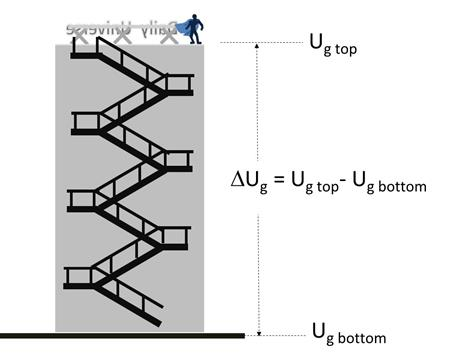
\includegraphics[width=2.8in,height=2.5in]{PH4CAU1I}
\end{figure}

Because voltage is proportional to a \emph{difference} in electrical potential energy, a voltage measurement really is a combination of two measurements. Think of gravitational potential energy. If we ask for the potential energy difference as Super Guy jumps from the bottom of a building to the top we need two measurements, one at the bottom and one at the top. Then 

\begin{equation*}
	\Delta U_{g}=U_{g_{top}}-U_{g_{bottom}}
\end{equation*}

We will do something very similar in measuring voltages. We will measure the potential energy at two places. For example, suppose we have an electric circuit as shown in the next figure. 

\begin{figure}[h!]
	\centering	
    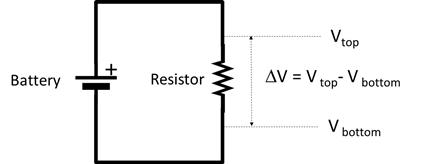
\includegraphics[width=3.5466in,height=1.3932in]{PH4CAU1J}
\end{figure}

The circuit is very simple, just a battery and a resistor. You have experience with batteries, and resistors now. A resistor is just a piece of material that has lots of electrical friction, or ``resistance'' that makes it hard for electrons to go through it. If we want to measure the voltage across the resistor, we have to measure on the top and bottom of the resistor. That will give us a measurement proportional to the potential energy difference from one side to the other of the resistor.

Most meters that measure voltage have two ``probes'' and do the difference calculation internally. These meters are called \emph{voltmeters} and we used them last week.

\begin{figure}[h!]
	\centering
	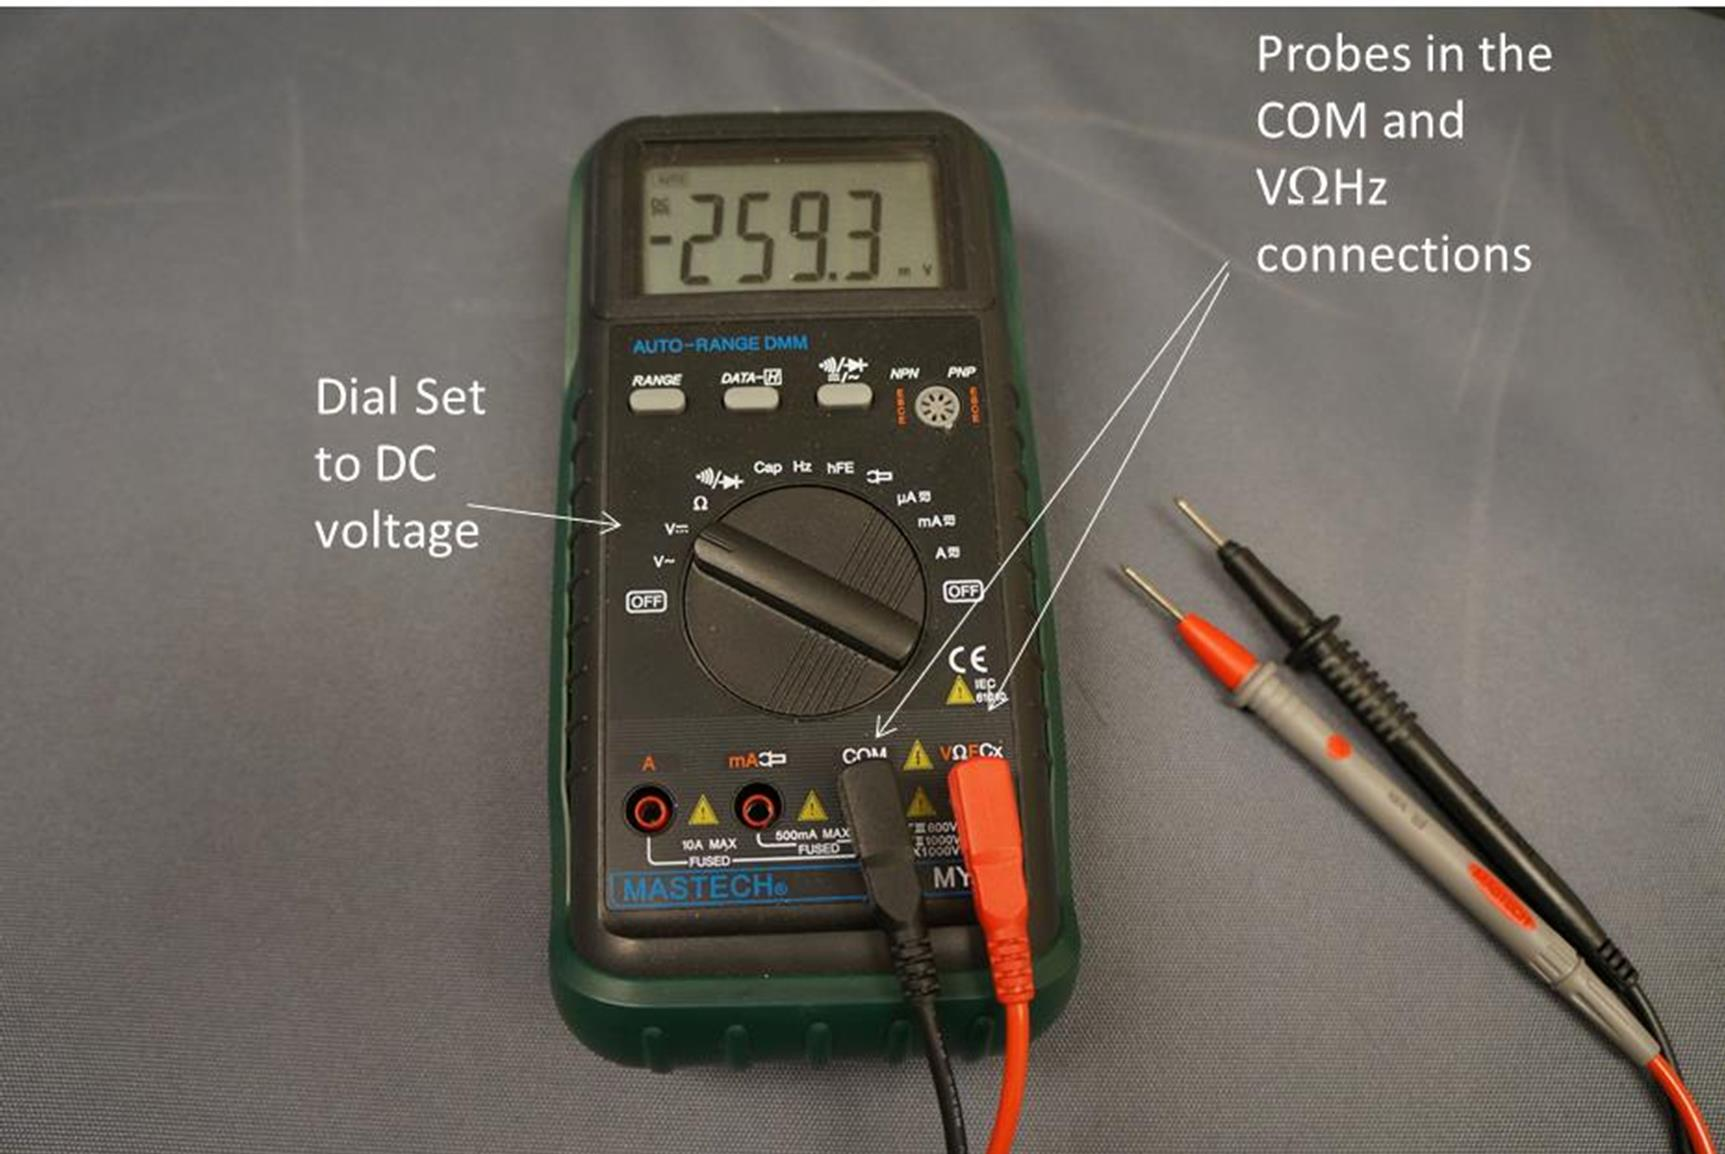
\includegraphics[width=2.9199in,height=1.962in]{PH4CAU1K}
\end{figure}

In today's world, voltmeters are usually just one part of a device that can measure many things. We call these devices multimeters. To measure voltage we will set the multimeter on the DC Voltage setting. Notice the two probe wires in the figure. We need two probes to make the two measurements and the device does the subtraction for us.

We learned to use a sand-alone voltmeter in the last lab. But we also need to read in voltages in a way that the data shows up on our computer. To get the data into our computer we will use a different set of pins on our Arduino board. They are called \emph{analog} pins.

Even before we begin, we need a warning. We absolutely must not wire up the analog pins on our Arduino backwards! This can (and probably will) destroy the pin circuitry inside our Arduino. So we will need to be careful in wiring for this part of our lab. Where this could be a problem a warning sign will appear in the text, just to remind you to be careful! 

\begin{figure}[h!]
	\centering
	
\includegraphics[width=2.8089in,height=1.4684in]{PH4CAU1L}
\end{figure}

You may see quite a few of these in this lab.

\section{Building a voltmeter}

Our Arduino has what we call and Analog to Digital converter (ADC). That is, it takes analog voltage signals that could have any value, and it maps them into a set of discrete values and sort of rounds to the nearest whole discrete value.

The word ``analog'' might not be familiar. Think of our power supply. It has a knob that adjusts the voltage. The knob can produce any voltage from $0$ to about $30\unit{V}$. This is an analog signal. The voltage can take on any value in a range. So we represent an analog signal with real numbers and we might have a voltage of exactly 

\begin{equation*}
	4.3276854325532573457\unit{V}
\end{equation*}

\noindent and this would be perfectly valid for an analog signal.

A battery, on the other hand, is not this way. It has a fixed voltage, say, $1.5\unit{V}$ like the D-Cell batteries that we used in our last lab. Two D-Cell batteries could be used together to make $3\unit{V}.$ But you can't use D-Cell batteries to get $2.25\unit{V}.$ The batteries come in discrete units.

Our Arduino analog pin is designed to measure voltages in the range $0$ to $5\unit{V}.$ Don't set your power supply to more than $5\unit{V}!$ But there is more to the ADC than just a voltage range. The Arduino chops the voltage range into 1024 discrete voltage divisions. Each division is then

\begin{equation*}
	\Delta v_{\min }=\frac{5\unit{V}}{1024}=4.\,\allowbreak 9\unit{mV}
\end{equation*}

\begin{figure}[h!]
	\centering
	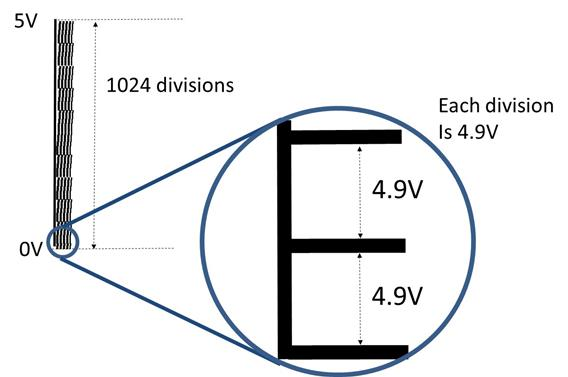
\includegraphics[width=2.3618in,height=1.5714in]{PH4CAU1M}
\end{figure} 

This means that changes in voltage that are less than $4.9\unit{mV}$ won't be seen, since it takes a whole $4.9\unit{mV}$ to get a different division. So if we give our Arduino $8\unit{mV}$ this is not enough to fill the second $4.9\unit{mV}$ division, so our Arduino would still read only $4.9\unit{mV}.$ If we gave it $11\unit{mV}$ it would then read $9.8\unit{mV}$ because $9.8\unit{mV}=2\times 4.9 \unit{mV}$ and $9.8$ is the closest whole unit of $4.9\unit{mV}.$

\begin{figure}[h!]
    \centering
    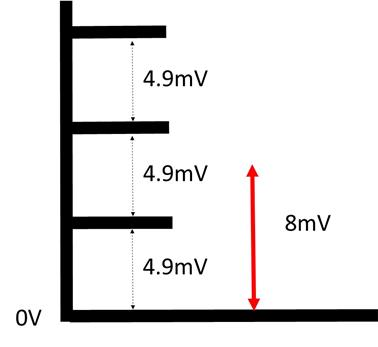
\includegraphics[width=3.1868in,height=2.9265in]{PH4CAU1N}
\end{figure}

This is called ``discretization'' or more commonly ``digitization'' or even \emph{``quantization.'' } We have taken a signal that might have any value between $0$ to $5\unit{V}$ and we output a signal that will be rounded to the nearest $n\times 4.9\unit{mV}.$

As a second example, $3.793\unit{V}$ would be reported as $\allowbreak 3.792\,\allowbreak 6\unit{V}$ since 

\begin{equation*}
	\frac{3.793\unit{V}}{4.9\unit{mV}}=774.\,\allowbreak 08
\end{equation*}

\noindent but we need even units of $\Delta v_{\min },$ so the $0.8$ would be dropped by the A2D converter giving 

\begin{equation*}
	774\times 4.9\unit{mV}=\allowbreak 3.792\,\allowbreak 6\unit{V}
\end{equation*}

\noindent and our first voltage from our power supply, $4.3276854325532573457\unit{V}$ would be reported as $4.\,\allowbreak 326\,7\unit{V}$ (make sure you can see how we got this result!).

This means that we can be off in our voltage measurements as much as $4.9\unit{mV}$! In dividing up our voltage range into $1024$ pieces we have introduced some error, but we have divided our $0$ to $5\unit{V}$ into numeric values that we can use in our computer, so it is worth the cost of some error.

The amount of error depends on how many different values the ADC converter has. Since breaking an analog signal into discrete values is called \emph{quantization, }we call this source of error \emph{quantization error.} It is the source of much of the error we see in electronic measuring devices. We could say that our new voltmeter has an uncertainty of at least the voltage resolution

\begin{equation*}
	\delta V_{signal}=\Delta V_{\min }=4.\,\allowbreak 9\unit{mV}
\end{equation*}

\noindent but of course it could be larger if there are other sources of error.

The ADC sends the measured value through our USB cable to our computer's serial port. But it doesn't send it in units of volts. It sends it in ADC units. If we have a signal voltage of $9.8\unit{mV}$ we don't get out $9.8,$ we get $2$ because $9.8\unit{mV}=2\Delta V_{\min }.$ The ADC units are the number of $\Delta V_{\min }$ sized units that are in our signal voltage. To get back to voltage units, we need to multiply by $\Delta V_{\min }.$ In our code we will do this before reporting the value. 

Of course we would like to see the voltage that we measure. There is a simple way to do this. The voltage values we calculate can be sent to our computer through the serial cable. We will need an Arduino sketch with some additional setup and some additional loop commands. One of these commands will turn our ADC units into volts. 

Before we look at the entire sketch, let me introduce the new commands that we will need. To get the Arduino to communicate with the computer we use the command 

\begin{equation*}
	\begin{tabular}{l}
		\ Serial.begin();
	\end{tabular}
\end{equation*}

\noindent and in the loop function we use the command

\begin{equation*}
	\begin{tabular}{l}
		\ Serial.print();
	\end{tabular}
\end{equation*}

We also need to know that computers make a distinction between integer and real numbers. Our voltages will be real numbers, so we need to tell the Arduino that we want a real number. The command for this is the word ``float.'' For example,

\begin{equation*}
	\begin{tabular}{l}
		\ float\ delta\_v\_min=0.0049;
	\end{tabular}
\end{equation*}

\noindent defines a variable named ``delta\_v\_min'' and sets it to the value $0.0049.$ If we want an integer number we use the word ``int.''  For example 

\begin{equation*}
	\begin{tabular}{l}
		\ int\ value\ =\ 0;
	\end{tabular}
\end{equation*}

\noindent defines a variable named ``value'' and sets it equal to $0.$ All this is a little like listing your variables back in PH121. Only here if you don't do it, it doesn't just cost you points, it confuses the Arduino software and the Arduino software will give you an error.

We also need special commands to read our Arduino analog pins. The special Arduino command 

\begin{equation*}
	\begin{tabular}{l}
		analogRead()
	\end{tabular}
\end{equation*}
will do this.

The whole Arduino sketch might look like this:
\href{https://dtoliphant.github.io/PH250Manual/Code/DAQ_voltmeter.ino}{Download here}
\lstinputlisting[language=Arduino]{Code/DAQ_voltmeter.ino}


Make sure you understand every line of this code. Write it in the Arduino IDE and run it to help see what the lines do. Lines that begin with two slashes, ``//,'' are comments. The Arduino will ignore these lines. But you shouldn't! The comments tell you, the programmer, what the code is doing. I will ask you in lab to input comments for every line. If there is any part of this sketch that is mysterious, work with your group to resolve the mystery and if it is still mysterious, call your instructor over to discuss the sketch with you.

\subsection{Wiring the simple voltmeter}

\begin{figure}[h!]
	\centering
	
\includegraphics[width=1.8507in,height=0.9677in]{PH4CAU1O}
\end{figure}

You knew that was coming, didn't you! We must be very careful to wire our Arduino correctly. Our Arduino can measure $0$ to $5\unit{V}.$ But if we switch the $5\unit{V}$ and the $0\unit{V}$ by plugging them into the wrong pin, our Arduino may be damaged and never work the same way again (probably won't work at all!). So wire first, then before you connect the Arduino have group member check your wiring, then check the wiring with a stand-alone meter (that is why we learned to use them last week). Also remember, more than $5\unit{V}$ will damage the Arduino. So only put in voltages in the range $0\unit{V}$ to $5 \unit{V}.$

We need one wire attached to the pin marked A0. We need another wire attached to one of our Arduino ground pins marked GND. And we connect the first wire to the positive output of our signal source (say, our power supply) and the GND wire to our negative output of our signal source (say the negative or ground connection on our power supply). That is all there is to it!

\subsection{Seeing the data}

Once the code is compiled and uploaded, the Arduino will send data to the serial port. The serial monitor can display the data. The serial monitor is found under the Arduino Software Tools menu on the legacy IDE, and down at the bottom hiding behind a tab in the new IDE.

\begin{figure}[h!]
	\centering
	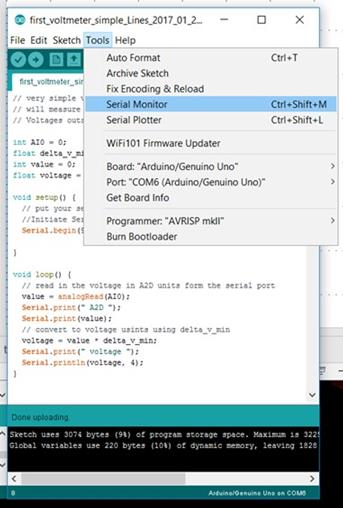
\includegraphics[width=2.0807in,height=3.0744in]{PH4CAU1P}
\end{figure}

\noindent You should see something like this:

\begin{figure}[h!]
	\centering
	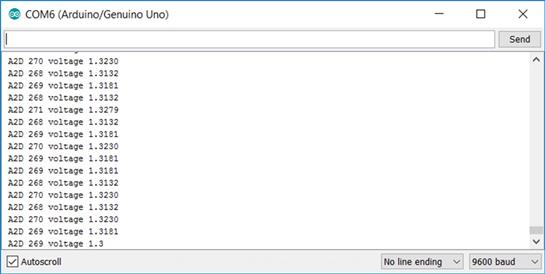
\includegraphics[width=4.5861in,height=2.3151in]{PH4CAU1Q}
\end{figure}

The Arduino Software can also plot the data from the serial port. In the next figure there is a plot of the same data that we saw on the serial monitor. 

\begin{figure}[h!]
	\centering
	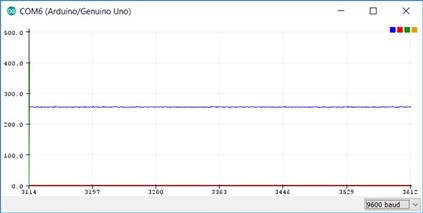
\includegraphics[width=3.563in,height=1.8049in]{PH4CAU1R}
\end{figure}

Notice that it plotted our voltage values and it also plotted our ADC values. This makes the voltage values hard to see. We could fix this by commenting out the lines that print the ADC values (putting ``//'' at the beginning of the line). Then those lines won't be executed by the Arduino. Then we get just the voltage. 

\begin{figure}[h!]
	\centering
    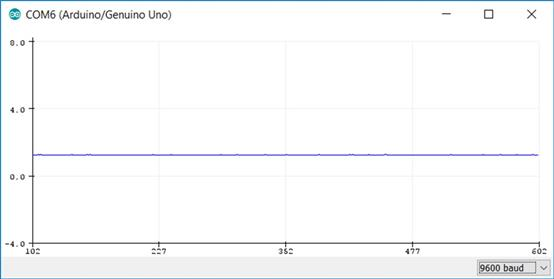
\includegraphics[width=3.2578in,height=1.6475in]{PH4CAU1S}
\end{figure}

Notice that the horizontal axis is not exactly time. It is just the data point number. We could convert this to time with some calculation if we know how often the Arduino sends us a data point. I will leave this as an exercise.

\section{Extending our voltmeter with a voltage divider\label{Voltmeter with Voltage Divider}}



This Arduino-based voltmeter that we have built is great, but will only let us measure voltages in the range $0$ to $5\unit{V}.$ That seems a little restrictive. We would like to extend our voltmeter to a larger range, say, $0 $ to $20\unit{V}.$ To do this, we will need to add some electronic components and think about what we have learned about voltage, resistance, and current. Let's consider this circuit.

\begin{figure}[h!]
	\centering
	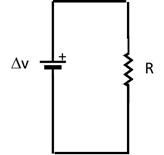
\includegraphics[width=1.3932in,height=1.1188in]{PH4CAU1T}
\end{figure}

\vspace{1in} % to keep the figure in the right spot in the text

\noindent We have a battery, That will make the current flow much like a pump makes water move through pipes.

\begin{figure}[h!]
	\centering
	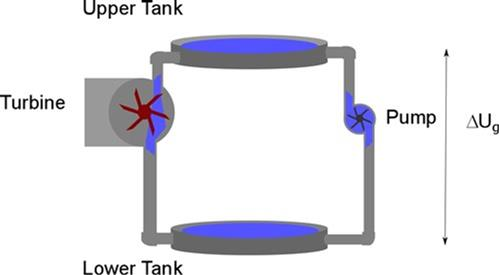
\includegraphics[width=4.2004in,height=2.3229in]{PH4CAU1U}
\end{figure}

The water in a pipe system gains potential energy as it moves up. In our circuit we will find that electric charge gains potential energy as we move it across a battery. Then the charge will move down the wire like water moves down a pipe until it is out of potential energy. Notice that the water in a pipe system will lose all the potential energy that it gained when the pump raised it to the upper tank (see previous figure). That is true of electric charge too. The electric current travels from the battery through the resistor, but in doing so it loses all the potential energy that the battery gave it by the time it returns to the battery.

Now suppose we have two resistors in a circuit.

\begin{figure}[h!]
	\centering
	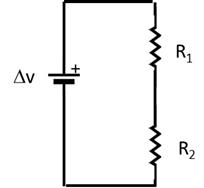
\includegraphics[width=1.7279in,height=1.1188in]{PH4CAU1V}
\end{figure}

\noindent Our water analogy can still help us understand what will happen. Suppose
that we have two turbines in our pipe system. 

\begin{figure}[h!]
	\centering
	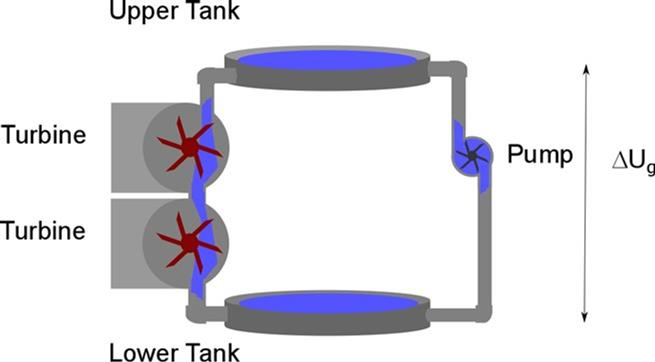
\includegraphics[width=3.5985in,height=1.9934in]{PH4CAU1W}
\end{figure}

The water leaves the high potential energy part of the pump, and is put to work turning the first turbine. The resistance of the turbine will slow the water current. So when the water leaves the turbine, it will have lost some potential energy. Since we have a second turbine the current will again be slowed and more potential energy will be lost. How much potential energy do we lose as the water falls? All of the potential energy that the pump gave it! We must end up with the water at the bottom back at the low potential energy. We will find this to be true for our electric circuit as well. We will loose some potential energy as the electrical energy ``falls'' from the high electric potential ``down'' the first resistor. After the second resistor, we can guess that we must be back at the low electric potential we started with.

\begin{figure}[h!]
	\centering
	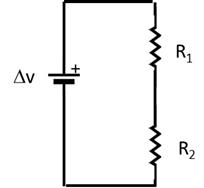
\includegraphics[width=1.7279in,height=1.5947in]{PH4CAU1X}
\end{figure}

We know that electric potential is a potential energy per unit charge. And energies just add up. If 

\begin{equation*}
	\Delta V=RI
\end{equation*}

\noindent is satisfied, then we would expect that adding two resistors would just linearly add the effects of the two resistors together

\begin{eqnarray*}
	\Delta V_{total} &=&\Delta V_{1}+\Delta V_{2} \\
	&=&R_{1}I+R_{2}I
\end{eqnarray*}

Note that the same current must flow through each of the resistors, since the current leaving $R_{1}$ is the current flowing into $R_{2}.$ Then 

\begin{equation*}
	\Delta V_{total}=\left( R_{1}+R_{2}\right) I
\end{equation*}

\noindent Our current will be 

\begin{equation*}
	I=\frac{\Delta V_{total}}{R_{1}+R_{2}}
\end{equation*}

But suppose we measure the potential change across just resistor $R_{2}.$ 

\begin{figure}[h!]
	\centering
	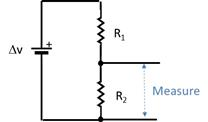
\includegraphics[width=1.7625in,height=1.0421in]{PH4CAU1Y}
\end{figure}

\noindent what would we expect to get? We lost voltage across both $\Delta V_{1}$ and $\Delta V_{2}$ so 

\begin{equation*}
	\Delta V_{total}=\Delta V_{1}+\Delta V_{2}
\end{equation*}

\noindent because we must loose all the $\Delta V_{total}$ given to the current by the
battery. And 

\begin{equation*}
	\Delta V_{2}=IR_{2}
\end{equation*}

\noindent from Ohm's law. So

\begin{equation*}
	\Delta V_{2}=\left( \frac{\Delta V_{total}}{R_{1}+R_{2}}\right) R_{2}
\end{equation*}

This is only part of the total voltage. And if we have two different resistors so that $R_{1}\neq R_{2}$ then we can choose for $\Delta V_{2}$ to be nearly as much as $\Delta V_{total}$ or nearly as little as $0$ by carefully choosing our two resistances. We call a set of two resistors like this a ``voltage divider'' because it divides the battery voltage between the two resistors. If $R_{1}$ is bigger than $R_{2}$ then $\Delta V_{1}$ is bigger than $\Delta V_{2}.$

Remember that the input can only withstand $0$ to $5\unit{V}.$ More than that can destroy the board! But we want to measure a voltage that varies from $0$ to $20\unit{V}.$ We now have a way to do this. We will use a voltage divider. The voltage across both resistors will be as much as $20\unit{V},$ but we will measure the voltage across only one of the resistors. And we will choose our resistor so that when the total voltage is $20\unit{V} $ but the voltage across our resistor is $5\unit{V}$ (or less). Since we will know the resistances, we can use a little math to calculate what the total voltage was using the voltage measurement from just one of the resistors.

This is like what we did to measure current last lab. We used a voltmeter and a resistor and some math to make an ammeter. Today we will use two resistors, our Arduino voltmeter, and some math to make a new voltmeter that can measure higher voltages. We just need to choose our resistors so that we
map our $0$ to $20\unit{V}$ to $0$ to $5\unit{V}.$ Once choice might be 

\begin{eqnarray*}
	R_{1} &=&40\unit{k \Omega} \\
	R_{2} &=&10\unit{k \Omega}
\end{eqnarray*}

\noindent Let's try it. We would get

\begin{eqnarray*}
	\Delta V_{2\max } &=&\left( \frac{20\unit{V}}{40\unit{k \Omega }
	+10\unit{k \Omega }}\right) \left( 10\unit{k \Omega }\right) \\
	&=&4.0\unit{V}
\end{eqnarray*}

\noindent when $\Delta V_{total}=20\unit{V}$ and 

\begin{eqnarray*}
\Delta V_{2\min } &=&\left( \frac{0\unit{V}}{40\unit{k \Omega}
	+10\unit{k\Omega}}\right) \left( 10\unit{k\Omega}\right) \\
	&=&0\unit{V}
\end{eqnarray*}

\noindent when $\Delta V_{total}=0\unit{V}.$ 
Notice that this really didn't work. We
only got a maximum voltage of $4\unit{V}.$ But this gives us a margin of safety. If we give our Arduino more than $5\unit{V}$ we can burn it up. If we plan our circuit so we don't get to close to $5\unit{V}$ we are safer. So this set of resisters is not a terrible choice.

To report out our voltage we need to do this conversion backwards. Say we have $\Delta V_{total}=10\unit{V}$ that we are measuring with our new instrument. Then 

\begin{eqnarray*}
	\Delta V_{2} &=&\left( \frac{10\unit{V}}{40\unit{k \Omega}
	+10\unit{k\Omega}}\right) \left( 10\unit{k\Omega}\right) \\
	&=&2\unit{V}
\end{eqnarray*}

The $2\unit{V}$ is what we actually measure at the A0 input. But we know
that this represents $10\unit{V}$ across both resistors, so we want the
Arduino program to print out $10\unit{V}.$ So we report

\begin{equation*}
	\Delta V_{reported}=\frac{\Delta V_{2}}{R_{2}}\left( R_{1}+R_{2}\right)
\end{equation*}

\noindent or for our case, since we measured $2\unit{V}$ across our resistor,

\begin{equation*}
	10\unit{V}=\frac{2\unit{V}}{\left( 10\unit{k\Omega}\right) }\left( 40\unit{k\Omega}+10\unit{k\Omega}\right)
\end{equation*}

We will have to write this math in our code. There is a further complication. The Arduino A0 input is giving us a number that represents $0$ to $4\unit{V}$ for our setup. But that is not what we see on the serial port. We see a number from 0 to 1024. We know the $1024$ represents $5\unit{V}$ and the $0$ represents $0\unit{V}.$ So we need to multiply the number that comes from our Arduino by $\delta V=4.9\unit{mV}$ once again to get our Arduino output into voltage units. So our reported voltage equation is something like this. 

\begin{equation*}
	\Delta V_{reported}=A2D\times \delta V_{2}\times \frac{1}{R_{2}}\left(R_{1}+R_{2}\right)
\end{equation*}

All this calculation to get our reported voltage must do something to our measurement uncertainty. We could do our usual math to find the reported uncertainty, but instead, let's think. Every small voltage $\Delta V_{2}$ would be multiplied by $\left( \frac{1}{R_{2}}\left( R_{1}+R_{2}\right) \right) $ to map it into our original $0\unit{V}$ to $20\unit{V}$ range. That should work for our smallest voltage that we can detect, namely $\delta V=4.9\unit{mV}.$ That is the smallest value $\Delta V_{2}$ could have. So in our $0\unit{V}$ to $20\unit{V}$ range the smallest value this can map to is  

\begin{equation*}
	\delta V_{reported}=\left( \delta V\right) \left( \frac{1}{R_{2}}\left(R_{1}+R_{2}\right) \right)
\end{equation*}

The first term in parenthesis is essentially $1$ digitizer unit multiplied by $\Delta V_{2}$ and the second term in parenthesis converts the $\Delta V_{2}$ value into actual volts measured across both resistors.

The quantity $\delta V_{reported}$ gives us our quantization error value for our new instrument. Our output will be in multiples of 

\begin{equation*}
	V_{reported}=n\times \delta V_{reported}
\end{equation*}

\noindent Putting in numbers gives 

\begin{eqnarray*}
	\delta V_{reported} &=&\left( 4.\,\allowbreak 884\times 10^{-3}\unit{V} \right) \left( \frac{1}{10\unit{k\Omega}}\left( 40\unit{k\Omega}+10\unit{k\Omega}\right) \right) \\
                        &=&0.024\,42\unit{V} \\
                        &=&24.42\unit{mV}
\end{eqnarray*}

This is much bigger than our $4.9\unit{mV}$ uncertainty for the simple voltmeter. And this is the cost of using a voltage divider to extend our voltage range. For the bigger voltage range we get a bigger uncertainty.

Let's try another example. Suppose we wish to measure $0$ to $20\unit{V}$ and we look in our case of resistors and find we have the following two resistors to use:

\begin{eqnarray*}
	R_{1} &=&98\unit{k\Omega} \\
	R_{2} &=&15\unit{k\Omega}
\end{eqnarray*}

We would expect that our $0$ to $20\unit{V}$ would be mapped to a smaller range. Let's find that range.

\begin{eqnarray*}
	\Delta V_{2\max } &=&\left( \frac{20\unit{V}}{98\unit{k\Omega}+15\unit{k\Omega}}\right) \left( 15\unit{k\Omega}\right) \\
                      &=&2.\,\allowbreak 654\,9\unit{V}
\end{eqnarray*}

So our voltage range at the Arduino A0 input will be $0\unit{V}$ to $ 2.\,\allowbreak 65\unit{V}.$ This set of resistors won't use the full Arduino $0\unit{V}$ to $5\unit{V}$ range. But it will measure $0$ to $20 \unit{V}.$ The minimum detectable voltage for this new instrument design for
our $0$ to $20\unit{V}$ source will be 

\begin{eqnarray*}
	delta V_{reported} &=&\left( \delta V_{2}\right) \left( \frac{1}{R_{2}}\left( R_{1}+R_{2}\right) \right) \\
                       &=&\left( 4.\,\allowbreak 880\,3\times 10^{-3}\unit{V}\right) \left( \frac{1}{\left( 15\unit{k\Omega}\right) }\left( 98\unit{k\Omega}+15\unit{k\Omega}\right) \right) \\
                       &=&3.\,\allowbreak 676\,5\times 10^{-2}\unit{V} \\
                       &=&37\unit{mV}
\end{eqnarray*}

This uncertainty is much bigger than the uncertainty for our last choice of resistors. So $98\unit{k\Omega}$ and $15\unit{k\Omega}$ are not great choices even though they technically work.

For your version of the voltmeter in lab, you will choose the resistor values to use. Here is an Arduino sketch to implement this extended volt meter. In it are the not-so-good $98\unit{k\Omega}$ and $15\unit{k\Omega},$ but of course \textbf{you should change the sketch to have your resistor
values}.

\href{https://dtoliphant.github.io/PH250Manual/Code/DAQ_Extended_voltmeter.ino}{Download here}
\lstinputlisting[language=Arduino]{Code/DAQ_Extended_voltmeter.ino}


\bigskip Of course you will want to have another person check your math and
wiring, and you should check your output voltage with a stand-alone meter
before you plug into your Arduino.

\section{Practice Problems}

\rule{11cm}{0.03cm}

Here is an example for you to work out on your own before class. Do this and compare your result to the results of the other people in your lab group as you come into class on lab day.

Suppose we wish to measure $0$ to $15\unit{V}$ and we look in our case of resistors and find we have the following two resistors to use:

\begin{eqnarray*}
	R_{1} &=&43.2\unit{k\Omega} \\
	R_{2} &=&15.2\unit{k\Omega}
\end{eqnarray*}

What range of voltages would we see at the Arduino, and what is the quantization error for our measurement?

\rule{11cm}{0.03cm}

%%%%%%%%%%%%%%%%%%%%%%%%%%%%%%%%%%%%%%%%%%%%%%%%%%%%%%%%%%%%%%%%%%%%%%%%%%%%%%%%%%%%%%%%%%%%%%%
% Section on proposals goes here for block classes
%%%%%%%%%%%%%%%%%%%%%%%%%%%%%%%%%%%%%%%%%%%%%%%%%%%%%%%%%%%%%%%%%%%%%%%%%%%%%%%%%%%%%%%%%%%%%%%

\section{Proposals}

It's time to start thinking of what experiment you and your group will design. If you are taking PH250 as a block class we have to do this right at the start because it may take time to order in parts for your instrument that you will design. If you are taking PH250 as a full semester class, it is not as much of a hurry, but we still need lead time to order things. So even if it feels early, we need to think about this. You are required to write a proposal for this experiment. This is a document that is intended to persuade someone (your professor,  funding agency, yourself, etc.) that you should be given the resources and support to perform the experiment. The proposal consists of the following parts:

\begin{enumerate}
	\item Statement of the experimental problem
	
	\item Procedures and anticipated difficulties
	
	\item Proposed analysis and expected results
	
	\item Preliminary List of equipment needed
\end{enumerate}

\noindent Since you be writing each of these sections, let's discuss what should be in them.

\subsection{Statement of the experimental problem}

This is a physics class, so our experiment should be a physics experiment. The job of an experimental physicist is to test physics theory. So your statement of the experimental problem should include \textbf{what theory you are testing} and a brief, high level, overview of what you plan to do to test this theory.

\subsection{Procedures and anticipated difficulties}

Hopefully, your reader will be so excited by the thought of you testing your theory that he or she will want to know the details of what you plan to do. You should describe in some detail what you are planning. If there are hard parts of the procedure, tell how you plan to get through them.

\subsection{Proposed analysis and expected results}

You might think this is unfair. How are you supposed to know what analysis will be needed and what the results should be until you take the data? But really you both can, and should, make a good plan for your data analysis and figure out what your expected results should be. After all, you have a theory your are testing! You can encapsulate that theory into a predictive equation for your experiment. You can design your experimental apparatus, and put in the numbers from your experimental design. From this you can calculate what should be the outcome.

If you don't do this first, you don't know what equipment you will need or how sensitive that equipment needs to be. If you are trying to measure the size of your text book, an odometer that only measures in whole miles may not be the best choice of equipment. To know what you need, do the calculations in advance.

You should also do the error analysis. You will want to predict the uncertainty. A measurement of your laptop computer length that is good to $\pm 3\unit{m}$ is not very satisfying in most cases. Uncertainty in your result is governed by the uncertainty inherent in the measurements you will take. The uncertainty calculation tells you what sensitivity you will need in your measurement devices. Since you are choosing those measurement devices as part of your proposal, and you are choosing the inputs to your model equation (like the resistance and the capacitance in today's lab) you will know how much uncertainty they have, so you can do the calculation in advance.

You should do all of this symbolically if you can, numerically if you must, but almost never by hand (meaning don't use your calculator) giving single value results. Some measurements will come back poorer than you anticipated, or some piece of equipment will be unavailable. You don't want to have to redo all your calculations from scratch each time this happens. For example, in the event of an equipment problem, your analysis tells you if another piece of equipment is sufficiently sensitive, or if you need to find an exact replacement. When I perform an analysis like this, I try for a symbolic equation for uncertainty. I like to program these equations in Mathmatica, or Maple, or SAGE, or MathCAD, or whatever symbolic math processor I have. Alternately, you could code it into Python. Then, as actual measurements change, I instantly get new predictions. In the absence of a symbolic package, a spreadsheet program will do fine. A numerical program also is quick and easy to re-run with new numbers when no symbolic answer is found.

\subsection{Preliminary List of equipment needed}

Once you have done your analysis, you are ready to list the equipment you need and the sensitivity of the measurement equipment you need. Final approval of the project and the ultimate success of your experiment depend on the equipment you choose or are granted. You want to do a good job analyzing so you know what you need, and a good job describing the experiment so you are likely to have the equipment granted.

\subsection{Designing the Experiment}

Of course, as part of your proposal, you will have to design your experiment. In PH150 we learned that to design an experiment we needed the following steps. Some evidence of these steps should be found in your lab notebook:

\begin{enumerate}
	\item Identify the system to be examined. Identify the inputs and outputs. Describe your system in your lab notebook.
	
	\item Identify the model to be tested. Express the model in terms of an equation representing a prediction of the measurement you will make. Record this in your lab notebook.
	
	\item Plan how you will know if you are successful in your experiment. Plan graphs or other reporting devices. Record this in your lab notebook. This usually requires you to calculate the predicted uncertainty and to evaluate the relative size of the terms in the uncertainty equation (see below).
	
	\item Rectify your equation if needed. Record this in your lab notebook.
	
	\item Choose ranges of the variables. Record this in your lab notebook.
	
	\item Plan the experimental procedure. Record this in your lab notebook.
	
	\item Perform the experiment . Record this in your lab notebook (see next section).
\end{enumerate}

Let's just take a moment to recall what we learned from PH150 about group projects and lab notebooks.  You won't do all the work by yourself in a group project (we aren't in high school anymore!).  So you won't have an entry in your own lab notebook for everything that happens in your group project. For example, you might do the wiring, but someone else does the coding.  But if you say nothing about the coding, you have a huge hole in your record of what happened.  To solve this, you mention that the item happened (coding in our example) but just put in a reference to the person who did that part of the work.  So in our example you would put in a reference in your lab notebook to the lab notebook of the person who wrote the code.  That way, in your work group there is a clear path to what was done in everyone's lab notebooks.  This is what you do in real jobs!  So we will practice it here (and yes, it gets graded, because this isn't a real job, just a class).

\subsection{Using Uncertainty to refine experimental design.}

Suppose you plan to test our model for resistance from your PH220 text book. The equation for resistance is 

\begin{equation*}
	R=\rho \frac{\ell }{A}
\end{equation*}

\noindent where $\rho $ is the resistivity, the material properties of the material that makes wire or resistor have friction. The length of the wire or resistor is $\ell $, and $A$ is the cross sectional area. We could find the uncertainty in $R$

\begin{equation*}
	\delta R=\sqrt{\left( \frac{\partial R}{\partial \rho }\delta \rho \right)
		^{2}+\left( \frac{\partial R}{\partial \ell }\delta \ell \right) ^{2}+\left( 
		\frac{\partial R}{\partial A}\delta A\right) ^{2}}
\end{equation*}

\noindent The first term in the square root is 

\begin{equation*}
	\left( \frac{\partial R}{\partial \rho }\delta \rho \right) ^{2}=\left( 
	\frac{\ell }{A}\delta \rho \right) ^{2}
\end{equation*}

\noindent and the other two terms are 

\begin{equation*}
	\left( \frac{\partial R}{\partial \ell }\delta \ell \right) ^{2}=\left( 
	\frac{\rho }{A}\delta \ell \right) ^{2}
\end{equation*}

\begin{equation*}
	\left( \frac{\partial R}{\partial A}\delta A\right) ^{2}=\left( -\rho \frac{%
		\ell }{A^{2}}\delta A\right) ^{2}
\end{equation*}

And suppose that our design is to have a copper wire with 

\begin{eqnarray*}
	\rho &=&1.68\pm 0.03\times 10^{-8}\unit{\Omega}\unit{m} \\
	\ell &=&5.0\pm 0.1\unit{m} \\
	A &=&5.0\times 10^{-10}\unit{m}^{2}\unit{m}^{2}
\end{eqnarray*}

\noindent This would give a resistance of 

\begin{eqnarray*}
	R_{new} &=&1.68\times 10^{-8}\unit{\Omega}\unit{m}\frac{5\unit{m}}{5.0\times 10^{-10}\unit{m}^{2}} \\
	&=&168.0\unit{\Omega}
\end{eqnarray*}

We can calculate each of our terms from the $\delta R$ equation. 

\begin{equation*}
	\left( \frac{\ell }{A}\delta \rho \right) ^{2}=\left( \frac{5\unit{m}}{%
		5.0\times 10^{-10}\unit{m}^{2}}\left( 0.03\times 10^{-8}\unit{\Omega	}\unit{m}\right) \right) ^{2}=9.0\unit{\Omega}^{2}
\end{equation*}

\begin{equation*}
	\left( \frac{\rho }{A}\delta \ell \right) ^{2}=\left( \frac{1.68\times
		10^{-8}\unit{\Omega}\unit{m}}{5.0\times 10^{-10}\unit{m}^{2}}\left( 0.1\unit{m}\right) \right) 	^{2}=11.\,\allowbreak 290\unit{\Omega}^{2}
\end{equation*}

\begin{equation*}
	\left( -\rho \frac{\ell }{A^{2}}\delta A\right) ^{2}=\left( -\left(
	1.68\times 10^{-8}\unit{\Omega}\unit{m}\right) \frac{\left( 5\unit{m}\right) }{\left( 5.0\times 10^{-10} \unit{m}^{2}\right) ^{2}}\left( 0.1\times 10^{-9}\unit{m}^{2}\right) \right)
	^{2}=1129.\,\allowbreak 0\unit{\Omega}^{2}
\end{equation*}

\noindent The overall uncertainty then would be

\begin{equation*}
	\delta R=\sqrt{9.0\unit{\Omega}^{2}+11.\,\allowbreak 290\unit{\Omega}^{2}+1129.\,\allowbreak 0\unit{\Omega}^{2}}=33.\,\allowbreak 901\unit{\Omega}
\end{equation*}

So with this design we predict a fractional uncertainty of 

\begin{equation*}
	\frac{33.\,\allowbreak 901\unit{\Omega}}{168.0\unit{\Omega}}=0.201\,79
\end{equation*}

or a little over $20\%.$ This is not a great design. We would like a much lower uncertainty, something that gives a fractional uncertainty more like $1\%.$ It is clear that the last term has the highest contribution to the uncertainty, so this is the term that needs fixing. One method of fixing the problem would be to decrease $A.$ We could try $1.0\pm 0.1\times 10^{-9}\unit{m}^{2}.$ In order to have the same resistance we will also have to change the length of the wire from $10\unit{m}$ to $5\unit{m}$. 

\begin{eqnarray*}
	\rho &=&1.68\pm 0.03\times 10^{-8}\unit{\Omega}\unit{m} \\
	\ell &=&10.0\pm 0.1\unit{m} \\
	A &=&1.0\pm 0.1\times 10^{-9}\unit{m}^{2}
\end{eqnarray*}

Checking we see we do get the same resistance 

\begin{eqnarray*}
	R &=&1.68\times 10^{-8}\unit{\Omega	}\unit{m}\frac{10\unit{m}}{1.0\times 10^{-9}\unit{m}^{2}} \\
	&=&168\unit{\Omega}
\end{eqnarray*}

\noindent But now for the last term we would get 

\begin{equation*}
	\left( -\rho \frac{\ell }{A^{2}}\delta A\right) ^{2}=\left( -\left(
	1.68\times 10^{-8}\unit{\Omega}\unit{m}\right) \frac{\left( 10\unit{m}\right) }{\left( 1.0\times 10^{-9}\unit{m}^{2}\right) ^{2}}\left( 0.1\times 10^{-9}\unit{m}^{2}\right) \right)^{2}=282.\,\allowbreak 24\unit{\Omega}^{2}
\end{equation*}

\noindent which is better. But we have to check to make sure our design change didn't
cause a large rise in the other two terms. 

\begin{equation*}
	\left( \frac{\ell }{A}\delta \rho \right) ^{2}=\left( \frac{10\unit{m}}{		1.0\times 10^{-9}\unit{m}^{2}}\left( 0.03\times 10^{-8}\unit{\Omega}\unit{m}\right) \right) ^{2}=9.0\unit{\Omega}^{2}
\end{equation*}

\begin{equation*}
	\left( \frac{\rho }{A}\delta \ell \right) ^{2}=\left( \frac{1.68\times
		10^{-8}\unit{\Omega}\unit{m}}{1.0\times 10^{-9}\unit{m}^{2}}\left( 0.1\unit{m}\right) \right)^{2}=2.8224\unit{\Omega}^{2}
\end{equation*}

The first term was hurt by our new design change, but not badly. So with the new design the overall uncertainty would be 

\begin{equation*}
	\delta R=\sqrt{9.0\unit{\Omega}^{2}+2.8224\unit{\Omega}^{2}+282.\,\allowbreak 24\unit{\Omega		}^{2}}=17.\,\allowbreak 148\unit{\Omega}
\end{equation*}

\noindent So with this new design we predict a fractional uncertainty of

\begin{equation*}
	\frac{17.\,\allowbreak 148\unit{\Omega}}{168.0\unit{\Omega	}}=0.102\,07
\end{equation*}

which is about $\allowbreak 10.\%.$ This is much better. From our uncertainty terms, we can see that to do better we need to improve both the $\delta A$ term and the $\delta \ell $ terms because they are now about the same size. Probably no one in our class is really testing the resistance equation. This is just an example. But the point we need to take away from this example is that \textbf{the terms in our uncertainty calculation tell us how to modify our experimental design.}

There is a refinement we could make to our process. really there are no area measurement devices available, so what we would do is measure the diameter of the wire and calculate the area.

\begin{equation*}
	A=\frac{1}{4}\pi D^{2}
\end{equation*}

We could find $\delta A$ by using our propagation of uncertainty equation again, or we could modify our resistance equation so that it is in terms of what we actually measure.

\begin{equation*}
	R=\rho \frac{4\ell }{\pi D^{2}}
\end{equation*}

\noindent and calculate our uncertainty in terms of $\rho ,$ $\ell ,$ and $D.$ That is preferred and usually less work. The general rule is to express your model equation in terms of what you will actually measure before you calculate the uncertainty terms.

The moral of this long story is that we must calculate the uncertainty \textbf{ \emph{as part of the design process} }. It is probably best to use a symbolic math processor or at lease a python program or spreadsheet so that as the design changes your uncertainty estimate will change too without having to manually recalculate it.




%%%%%%%%%%%%%%%%%%%%%%%%%%%%%%%%%%%%%%%%%%%%%%%%%%%%%%%%%%%%%%%%%%%%%%%%%%%%%%%%%%%%%%%%%%%%%%%

\vspace*{\fill}

\pagebreak

\section{Lab Assignment}

\begin{enumerate}
	\item \textbf{Simple Arduino Voltmeter}

	\begin{enumerate}
		\item Build a circuit with one of our power supplies and a resistor like we did in our last lab. You can choose any resistor. (see section (\ref{Voltage Measurement with Meter}). 
			\begin{figure}[h!]
				\centering
				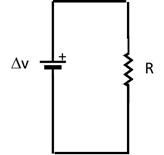
\includegraphics[width=1.3932in,height=1.3188in]{PH4CAU1Z}
			\end{figure}

			
			\begin{figure}[h!]
				\centering
				
\includegraphics[width=1.07in,height=0.5677in]{PH4CAU20}
			\end{figure}

			This time write the simple voltmeter sketch, wire it up, and measure the voltage across the resistor using our Arduino and the serial monitor. Be careful to stay in the $0$ to $5\unit{V}$ range!

		\item Calculate the uncertainty due to quantization error for your Arduino
			simple voltmeter

		\item Compare your calculated uncertainty to the measured uncertainty that
			you see in your device output. (This is tricky, does the power supply give a truly constant voltage?)
	\end{enumerate}

	\item \textbf{Build a new extended Voltmeter Using a Voltage Divider}

		\begin{enumerate}
			\item Build the voltage divider using two resistors as described in  section. (\ref{Voltmeter with Voltage Divider}). You will have to think about which resistors from our set will work best. Discuss this with your group, or have group members try the calculations with different combinations.
			
			\begin{figure}[h!]
				\centering
				
\includegraphics[width=1.07in,height=0.5677in]{PH4CAU21}
			\end{figure}

			\item Use a multimeter to verify that the output of the voltage divider is
			never more than $5\unit{V}$ and never less than $0\unit{V}.$ Take your power supply all the way from $0\unit{V}$ to $20\unit{V}$ and watch the multimeter to ensure it stays in the $0$ to $5\unit{V}.$ Range.\textbf{\ Do this with a multimeter before you hook up your Arduino.} You are making sure everything works so you won't destroy your Arduino!

			\item 

				Write the sketch and then hook the output of your voltage divider to the A0 pin and the other side of $R_{2} $ to a GND pin.
				\begin{figure}[h!]
					\centering
					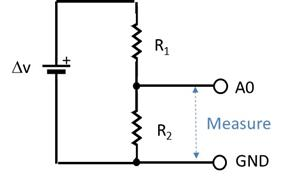
\includegraphics[width=2.3851in,height=1.5469in]{PH4CAU22}
				\end{figure}

				Your voltmeter should now be set up. Compile and load the sketch and use the Serial Plotter to watch the voltage values as you take the power supply from $0$ to $20\unit{V}$ using the serial monitor or plotter. \textbf{Don't go over }$20\unit{V}!$

				\item What is the quantization error for this voltmeter? Check to see if this matches your values on the serial monitor.

				\item Design a voltage divider that will allow the full $0$ to $30\unit{V}$ range of our power supply to be measured using the Arduino's $0$ to $5\unit{V}$ analog input. What would the quantization error be for this new circuit? 
		\end{enumerate}
	\item Together with your group, fill out a ``brainstorming sheet'' in preparation for your design project later in the semester.
\end{enumerate}